\StartPlate{V14}{A conductor filter is not an identification}{The critical-four candidate passes one invariant; it is not thereby identified with the source.}
\begin{center}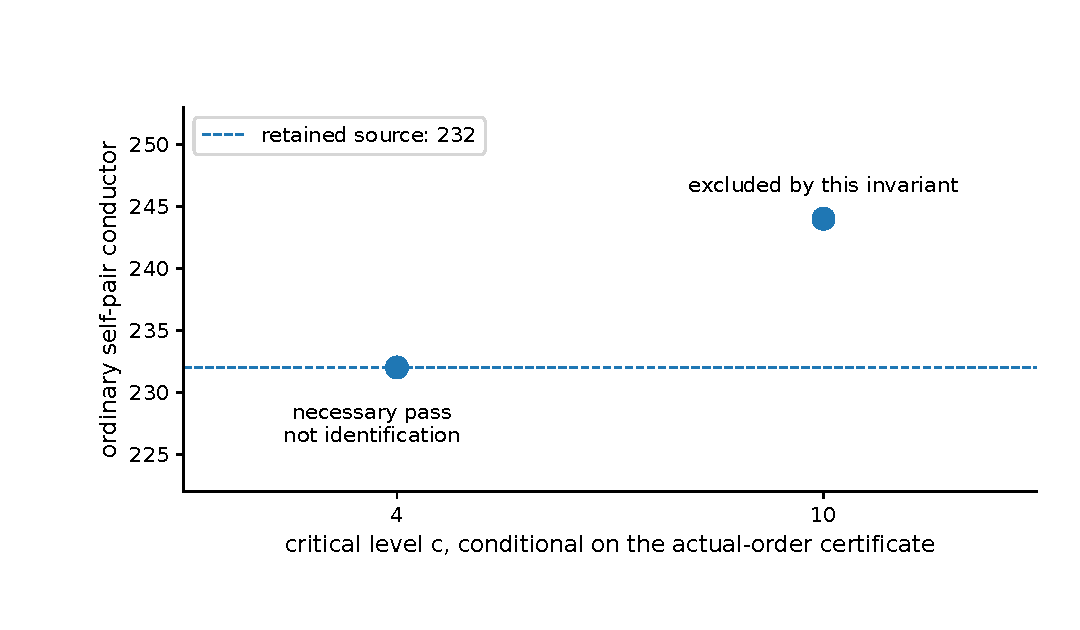
\includegraphics[width=\linewidth]{figures/V14.pdf}\end{center}
The two points use the recorded period-nine actual-order certificate. It gives leading level $24$, an even critical level $c$, index exponent $I=c+64$, and quotient dimension $D=8$. With the stipulated measures and torsion number one, the self-pair conductor is
\[
a(\pi^\vee\times\pi)=2c+224.
\]
At $c=10$ this is $244$, contradicting the unchanged source value $232$. At $c=4$ it is $232$, so this necessary comparison no longer excludes the candidate. The figure shows only these two conditional evaluations, not an asserted family of actual constructions for all intermediate values of $c$.

The order equations are substantive inputs. The pair $(24,c)$ does not imply them. Passing the horizontal line neither constructs the corrected stratum nor establishes occurrence of the complete prescribed character. Full pair-factor equality for the same candidate remains a stronger obligation than this conductor comparison.
\vfill\PlateSource{Conditional profile comparison}{Part III, Section 23.2--23.3}{60}
